\section{Power Optimized Software Envelope}
\label{sec:pose}

The POSE heuristic is based on the feasible performance envelope concept introduced in \autoref{sec:metrics}.
To build the feasible performance envelope for an invocation of code $\theta$ we first label the point corresponding to the observed runtime and energy costs of $\theta$.
We then plot lines of gradient $P_{max}$ and $P_{min}$ to represent the maximum and minimum bounds on energy consumption during normal operation of the target platform.
Lines of constant time and power draw are also added for the purpose of illustration.

At this point it is worth stating that our heuristic is a very general one.
It works for arbitrary metrics and is equally applicable at scales ranging from a single core to entire clusters.
Its only prerequisites are that accurate figures for energy and time can be obtained whilst running code on the system under investigation.

The broad applicability of POSE does raise the issue of how to find suitable maximum and minimum power boundaries for arbitrary systems. 
One approach is to rely on manufacturer supplied limits, however these values tend to be overly conservative approximations when they are available at all.
A better approach is to measure power consumption whilst the system executes some minimally expensive workload. 
The process of identifying such a workload is necessarily system specific and will be described further in \autoref{sec:investigation}.

To constrain our search space further we now consider the metric we wish to reduce. We know that for two invocations of logically equivalent codes $\theta$ and $\lambda$, the transformation $\theta \to \lambda$ is a valid optimization with respect to a cost metric $M$ if and only if $M(\lambda) < M(\theta)$. If we plot the curve linking all points having $M(\lambda) = M(\theta)$, then by definition any optimized versions of $\theta$ can only exist below this optimization bound.

Naturally the exact equation of the optimization bound depends on the metric chosen. 
The general form for the $E^mD^n$ family of metrics is derived as follows:
\begin{align}
E^mD^n(\theta) &= E^mD^n(\lambda) \nonumber \\
\implies {E_\lambda}^m &= \frac{{E_\theta}^m{D_\theta}^n}{{D_\lambda}^n} \nonumber \\
\implies E_\lambda &= (\frac{{E_\theta}^m{D_\theta}^n}{{D_\lambda}^n})^\frac{1}{m}
\end{align}

Our final bound considers what it means to optimize code for reduced power draw. We must avoid being too lenient; a large reduction in runtime associated with a negligible reduction in power draw should still be regarded as a classical optimization. On the other hand, our definition should include optimizations which deliver significant reductions in power draw with minuscule reductions in runtime. 

The definition we have settled on is that an optimization $\theta \to \lambda$ is a power optimization with respect to metric $M$ if the change in power draw it delivers is responsible for the majority of the reduction in $M$. Conversely, if the primary benefit of an optimization comes from improved runtime then it is to be considered a runtime optimization. We plot a curve linking those points which have the same ratio of contributions from both power and runtime factors to $M$ as our original code. All valid power optimizations must lie below this so-called contribution bound. 

Again the equation for the contribution bound depends on the metric chosen.
The general form for $E^mD^n$ metrics is derived as follows:
\begin{align}
\frac{{P_{\theta}}^m}{{D_{\theta}}^{m+n}} &= \frac{{P_{\lambda}}^m}{{D_{\lambda}}^{m+n}} \nonumber \\
\implies {P_{\lambda}}^m &= \frac{{P_{\theta}}^m}{{D_{\theta}}^{m+n}} \times {D_\lambda}^{m+n} \nonumber \\ 
\implies {E_{\lambda}}^m &= \frac{{P_{\theta}}^m}{{D_{\theta}}^{m+n}} \times {D_\lambda}^{m+n+1} \nonumber \\ 
\implies E_{\lambda} &= (\frac{{P_{\theta}}^m}{{D_{\theta}}^{m+n}} \times {D_\lambda}^{m+n+1})^{\frac{1}{m}} 
\end{align}

It may appear somewhat academic to base a bound on the definition of power optimization. That said, it is an important consideration in practice. Intuitively it makes sense to use the most appropriate tools while searching for optimizations.  If an optimization yields dramatic reductions in runtime with only minor reductions in power consumption then it is reasonable to state that conventional time-based profilers and performance engineering tools are better suited to finding it. The contribution bound enables our model to make this distinction.

\begin{figure}
\centering
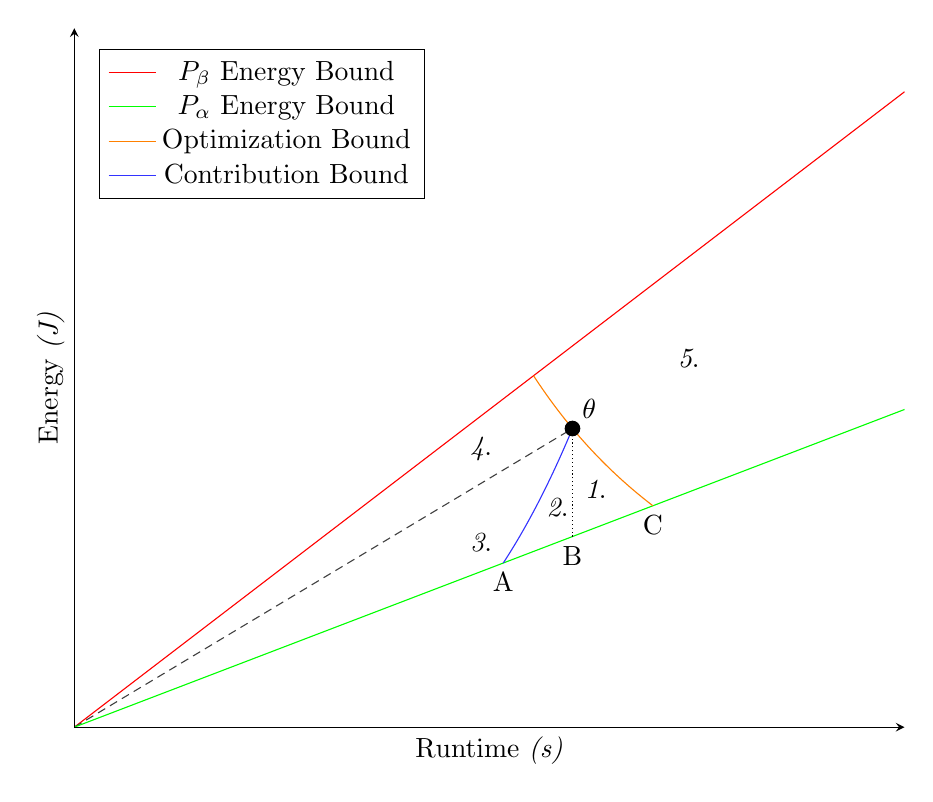
\begin{tikzpicture}
  \begin{axis}[ticks = none, 
    axis on top,
    axis x line=bottom,
    axis y line=left,
  	xlabel={Runtime \emph{(s)}},
    ylabel={Energy \emph{(J)}},    
    xmin=0, xmax=50,
    ymin=0, ymax=3300,
    width=\linewidth,
    legend style={legend pos=north west}
    ]

    %% Model Parameters %%
    \pgfmathsetmacro{\baselinepower}{30} % NOP code
    \pgfmathsetmacro{\rooflinepower}{60}
    \pgfmathsetmacro{\codepower}{47} 
    \pgfmathsetmacro{\codetime}{30}
    % Sadly, pgfplots sucks too much to calculate cube roots
    % These values are calculated with a ruby script in tools
    \pgfmathsetmacro{\anodex}{25.83028}
    \pgfmathsetmacro{\cnodex}{34.84283}
    \pgfmathsetmacro{\tnodex}{27.65477}

    \pgfmathsetmacro{\cnodey}{\cnodex * \baselinepower}
    \pgfmathsetmacro{\anodey}{\anodex * \baselinepower}
 
    %% Intermezzo Values %%
    \pgfmathsetmacro{\codeenergy}{\codepower * \codetime}
    \pgfmathsetmacro{\baselineenergy}{\baselinepower * \codetime}
    \pgfmathsetmacro{\rooflineenergy}{\rooflinepower * \codetime}
    \pgfmathsetmacro{\lowdisplayline}{(2 * \baselinepower + \codepower) / 3}
    \pgfmathsetmacro{\highdisplayline}{(1 * \rooflinepower + 1 * \codepower) / 2}

    % arguments: code power, code time, x - todo, apparently not supposed to do pgfmathparse
    \pgfmathdeclarefunction{metricbound}{3}{%
      \pgfmathparse{((#1 * #2^3) / #3^2)}%
    }
    \pgfmathdeclarefunction{definitionbound}{3}{%
      \pgfmathparse{((#1 / #2^3) * #3^4)}%
    }

    % BETA ROOFLINE BOUND
    \addplot[color=red, domain=\pgfkeysvalueof{/pgfplots/xmin}:\pgfkeysvalueof{/pgfplots/xmax}] {\rooflinepower * x};
    \addlegendentry{$P_{\beta}$ Energy Bound}

    %const power diagonal
    \addplot[color=darkgray, densely dashed, forget plot, %forget plot prevents legend entry
            domain=\pgfkeysvalueof{/pgfplots/xmin}:\codetime] {\codepower * x}; 

    % ALPHA BASELINE BOUND 
    \addplot[color=green, domain=\pgfkeysvalueof{/pgfplots/xmin}:\pgfkeysvalueof{/pgfplots/xmax}] {\baselinepower * x};
    \addlegendentry{$P_{\alpha}$ Energy Bound} 

    \addplot[color=orange, domain=\tnodex:\cnodex] { metricbound(\codepower, \codetime, x)};
    \addlegendentry{Optimization Bound}

    \addplot[color=blue!80, domain=\anodex:\codetime] { definitionbound(\codepower, \codetime, x)};
    \addlegendentry{Contribution Bound}

    % Constant Time, Energy Dashes
    %vertical
    \draw[densely dotted] ({axis cs:\codetime,\baselineenergy}) -- ({axis cs:\codetime,\codeenergy});

    \node[circle,fill,inner sep=2pt] at (axis cs:\codetime,\codeenergy) {};
    \node[above right] at (axis cs:\codetime,\codeenergy) {$\theta$};
    \pgfmathsetmacro{\oneycoord}{\lowdisplayline * 31.4}
    \node at (axis cs:31.4,\oneycoord) {\textit1.};
    \pgfmathsetmacro{\twoycoord}{\lowdisplayline * 29.1}
    \node at (axis cs:29.1,\twoycoord) {\textit2.};
    \pgfmathsetmacro{\threeycoord}{\lowdisplayline * 24.5}
    \node at (axis cs:24.5,\threeycoord) {\textit3.};
    \pgfmathsetmacro{\fourycoord}{\highdisplayline * 24.5}
    \node at (axis cs:24.5,\fourycoord) {\textit4.};
    \pgfmathsetmacro{\fiveycoord}{\codepower * 37}
    \node at (axis cs:37,\fiveycoord) {\textit5.};
    
    \node [below] at ({axis cs:\anodex, \anodey}) {A};
    \node [below] at ({axis cs:\codetime,\baselineenergy}) {B};
    \node [below] at ({axis cs:\cnodex, \cnodey}) {C};
    %\node [below, name intersections={of=metric bound and baseline}] at (intersection-1) {C};


 \end{axis}
\end{tikzpicture}

\caption{$ED^2P$ Code Optimization Space}
\label{fig:technique}
\end{figure}
The bounds described above allow us to identify the area of the Energy/Runtime plane in which power-optimized versions of a given code may exist. 
Along with lines of constant time and power draw, these bounds allow us to subdivide \autoref{fig:technique} into the following labelled areas:
\begin{enumerate}
\item Power-only optimizations
\item Power-mostly optimizations
\item Time-mostly optimizations
\item Time-only optimizations
\item Performance Degradation
\end{enumerate}


Despite its simplicity, this technique offers a wealth of information. The difference in energy between $\theta$ and intercept $B$ places an upper limit on the absolute amount of energy which can be saved by power optimization alone. The value $M(A) - M(\theta)$ bounds the amount of improvement in our metric we can expect to see from power optimization. The difference in runtime between intersect $C$ and $\theta$ represents the maximum increase in runtime we could feasibly trade off to achieve a slower yet more energy efficient code. Finally, the value $D(\theta) / D(A)$ represents the smallest speed-up which delivers more benefit than power optimization is capable of.

Only three measurements are required to build this plot; the system's baseline power draw, $P_{min}$, and the time and energy to solution for the code to be optimized, $D_\theta$ and $E_\theta$ respectively.
The precise value of $P_{max}$ can be ommitted when optimizing for power draw as we need not consider any values greater than our initial $P_\theta$.
We also need to consider which metric we are optimizing. \autoref{fig:technique} is based on $ED^2P$, whilst \autoref{fig:multimetric-technique} demonstrates how the POSE optimization area varies with metric choice.

\begin{figure}
\centering
\begin{tikzpicture}
  \begin{axis}[ticks = none, 
    axis on top,
    axis x line=bottom,
    axis y line=left,
  	xlabel={Runtime \emph{(s)}},
    ylabel={Energy \emph{(J)}},    
    xmin=0, xmax=50,
    ymin=0, ymax=3300,
    width=\linewidth,
    legend style={legend pos=north west}
    ]

    %% Model Parameters %%
    \pgfmathsetmacro{\baselinepower}{30} % NOP code
    \pgfmathsetmacro{\rooflinepower}{60}
    \pgfmathsetmacro{\codepower}{47} 
    \pgfmathsetmacro{\codetime}{30}




    %% Intermezzo Values %%
    \pgfmathsetmacro{\codeenergy}{\codepower * \codetime}
    \pgfmathsetmacro{\baselineenergy}{\baselinepower * \codetime}
    \pgfmathsetmacro{\rooflineenergy}{\rooflinepower * \codetime}
    \pgfmathsetmacro{\lowdisplayline}{(2 * \baselinepower + \codepower) / 3}
    \pgfmathsetmacro{\highdisplayline}{(1 * \rooflinepower + 1 * \codepower) / 2}

    % arguments: code power, code time, x, n 
    \pgfmathdeclarefunction{metricbound}{4}{%
      \pgfmathparse{((#1 * #2^(#4 + 1)) / #3^#4)}%
    }
    \pgfmathdeclarefunction{definitionbound}{4}{%
      \pgfmathparse{((#1 / #2^(#4 + 1)) * #3^(#4 + 2))}%
    }
 
    % BETA ROOFLINE BOUND
    \addplot[color=red, domain=\pgfkeysvalueof{/pgfplots/xmin}:\pgfkeysvalueof{/pgfplots/xmax}] {\rooflinepower * x};
    \addlegendentry{$P_{\beta}$ Energy Bound}

    %const power diagonal
    \addplot[color=darkgray, densely dashed, name path=constpwr, forget plot, %forget plot prevents legend entry
            domain=\pgfkeysvalueof{/pgfplots/xmin}:\codetime] {\codepower * x}; 

    % ALPHA BASELINE BOUND 
    \addplot[color=green, name path=basebound, domain=\pgfkeysvalueof{/pgfplots/xmin}:\pgfkeysvalueof{/pgfplots/xmax}] {\baselinepower * x};
    \addlegendentry{$P_{\alpha}$ Energy Bound} 

    % Constant Time vertical dots
    %vertical
    \draw[densely dotted] ({axis cs:\codetime,\baselineenergy}) -- ({axis cs:\codetime,\codeenergy});

    % Sadly, pgfplots sucks too much to calculate cube roots
    % Domain values are calculated with a ruby script in tools

    %% Energy Area %%
    \addplot[name path=energy, draw=none, domain=19.14894:47, forget plot]{ min(definitionbound(\codepower, \codetime, x, 0),metricbound(\codepower, \codetime, x, 0))};
    \addplot[blue!6] fill between[of=energy and basebound];
    \addlegendentry{Energy}

    %% Energy Delay Product Area %% 
    \addplot[name path=edp, draw=none, domain=23.96806:37.54997, forget plot] { min(definitionbound(\codepower, \codetime, x, 1),metricbound(\codepower, \codetime, x, 1))};
    \addplot[blue!13] fill between[of=edp and basebound];
    \addlegendentry{$EDP$}

    %% Energy Delay Squared Product Area ##
    \addplot[name path=edtwop, draw=none, domain=25.83028:34.84283, forget plot] { min(definitionbound(\codepower, \codetime, x, 2),metricbound(\codepower, \codetime, x, 2))};
    \addplot[blue!21] fill between[of=edtwop and basebound];
    \addlegendentry{$ED^2P$}

    %% Energy Delay Cubed Product Area ##
    \addplot[name path=edthreep, draw=none, domain=26.81496:33.56336, forget plot] { min(definitionbound(\codepower, \codetime, x, 3),metricbound(\codepower, \codetime, x, 3))};
    \addplot[blue!35] fill between[of=edthreep and basebound];
    \addlegendentry{$ED^3P$}




     \node[circle,fill,inner sep=2pt] at (axis cs:\codetime,\codeenergy) {};
    \node[above right] at (axis cs:\codetime,\codeenergy) {$\theta$};
  \end{axis}
\end{tikzpicture}

\caption{Multiple Metric Code Optimization Spaces}
\label{fig:multimetric-technique}
\end{figure}
